% Editable vector reconstruction of the supplied figure.
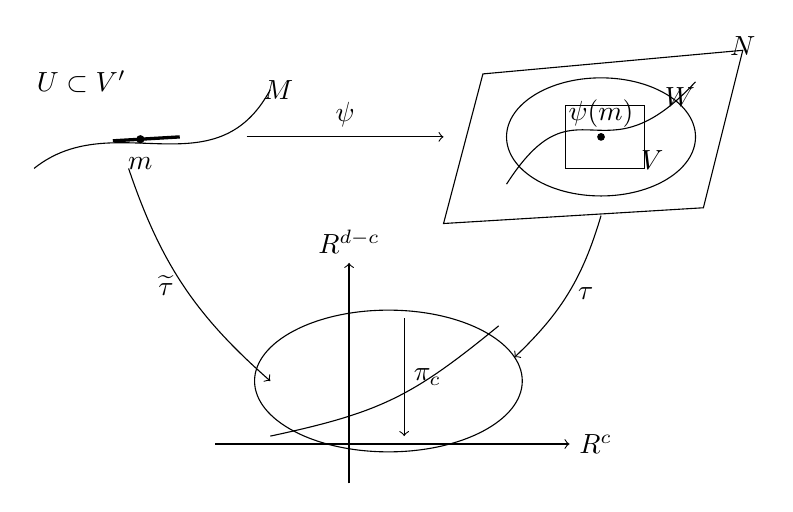
\begin{tikzpicture}
\draw(-.2,2)..controls(.8,2.8)and(2.1,1.7)..(2.8,3);\node at(2.9,3){$M$};\draw[line width=1.2pt](.8,2.35)--(1.65,2.4);\fill(1.15,2.37)circle(1.5pt)node[below=3pt]{$m$};\node at(.4,3.1){$U\subset V'$};
\draw(5,1.3)--(5.5,3.2)--(8.8,3.5)--(8.3,1.5)--cycle;\node at(8.8,3.55){$N$};\draw(7,2.4)ellipse(1.2 and .75);\node at(8,2.9){$W$};\draw(6.55,2)rectangle(7.55,2.8);\node at(7.65,2.1){$V$};\draw(5.8,1.8)..controls(6.7,3.2)and(7,1.8)..(8.2,3.1);\fill(7,2.4)circle(1.4pt)node[above]{$\psi(m)$};
\draw[->](2.5,2.4)--node[above]{$\psi$}(5,2.4);
\draw[->](3.8,-2)--(3.8,.8)node[above]{$\mathbb R^{d-c}$};\draw[->](2.1,-1.5)--(6.6,-1.5)node[right]{$\mathbb R^c$};\draw(4.3,-.7)ellipse(1.7 and .9);\draw(2.8,-1.4)..controls(4.2,-1.1)and(4.6,-.9)..(5.7,0);\draw[->](4.5,.1)--node[right]{$\pi_c$}(4.5,-1.4);
\draw[->](1,2)to[bend right=15]node[left]{$\widetilde\tau$}(2.8,-.7);\draw[->](7,1.4)to[bend left=15]node[right]{$\tau$}(5.9,-.4);
\end{tikzpicture}
